% University: Applied Science Private University

\documentclass{thesis-library}
\usepackage{array}
\usepackage{listings}
\renewcommand{\ttdefault}{lmtt}
\captionsetup{justification=centering}
\emergencystretch=1.5em
\newcommand{\tablefont}{\footnotesize\setstretch{1.15}\hyphenpenalty=10000\relax}
\newcolumntype{L}[1]{>{\raggedright\arraybackslash}p{#1}}
\lstset{
  basicstyle=\ttfamily\footnotesize,
  columns=fullflexible,
  keepspaces=true,
  frame=single,
  rulecolor=\color{gray!60},
  xleftmargin=2mm,
  xrightmargin=2mm,
  aboveskip=6pt,
  belowskip=6pt,
  breaklines=true,
  showstringspaces=false,
  upquote=true,
}

\begin{document}

\newcommand{\thesisTitle}{Cinema Ticket Reservation and Revenue Management System (CTRMS)\\[0.3cm]\large Phase 2: Design}
\newcommand{\byLabel}{By (Group 102):}
\newcommand{\studentName}{\begin{tabular}{c}Noureddin Ghazal (202511039)\\ Yousef Kitaneh (202311043)\\ Ahmad Jahaf (202310390)\end{tabular}}
\newcommand{\supervisorLabel}{Instructor:}
\newcommand{\supervisorName}{Dr. Khaled Al-Hashash}
\newcommand{\degreeLineALabel}{This project was submitted in Partial Fulfilment of the Requirements for the Microcomputer Systems and Assembly Language Course (1301224)}
\newcommand{\majorName}{}
\newcommand{\universityName}{Applied Science Private University}
\newcommand{\deanshipName}{Faculty of Information Technology}
\newcommand{\regionName}{Amman - Jordan}
\newcommand{\degreeyearName}{2026}
\newcommand{\degreemonthName}{November}

\makecoverpage

\pagenumbering{roman}

\newpage
\chapter*{\centering \Huge Table of Contents}
\addcontentsline{toc}{chapter}{Table of Contents}
\addtocontents{toc}{\protect\setcounter{tocdepth}{-1}}
\tableofcontents
\addtocontents{toc}{\protect\setcounter{tocdepth}{2}}

\newpage
\listoftablesname

\newpage
\listoffiguresname

\newpage
\pagenumbering{arabic}

% ── Chapter 1: Algorithm Design ─────────────────────────────────────────────

\printchaptertitle{Algorithm Design}

This chapter turns the process flows of the Phase 1 document into algorithms that can be coded directly in MASM. Every box that calls another procedure uses the procedure name defined in Chapter 3, and every field and array name is defined in Chapter 2. A box with double vertical edges is a call to another procedure. The register in brackets after a procedure name is the register that carries its parameter or its result, following the convention in Section~\ref{sec:params}.

\section{Main Program Flowchart}

\begin{minipage}{\textwidth}
The program initialises its data once, then repeats the menu cycle until the user chooses option 6. \texttt{DisplayMenu} only returns once it holds a valid choice from 1 to 6, so the dispatch chain in \texttt{main} never sees an invalid value. Every operation ends with the Irvine32 \texttt{WaitMsg} routine (\texttt{Press any key to continue...}) so the user can read the result before the screen is cleared for the next menu.

\medskip
\centering
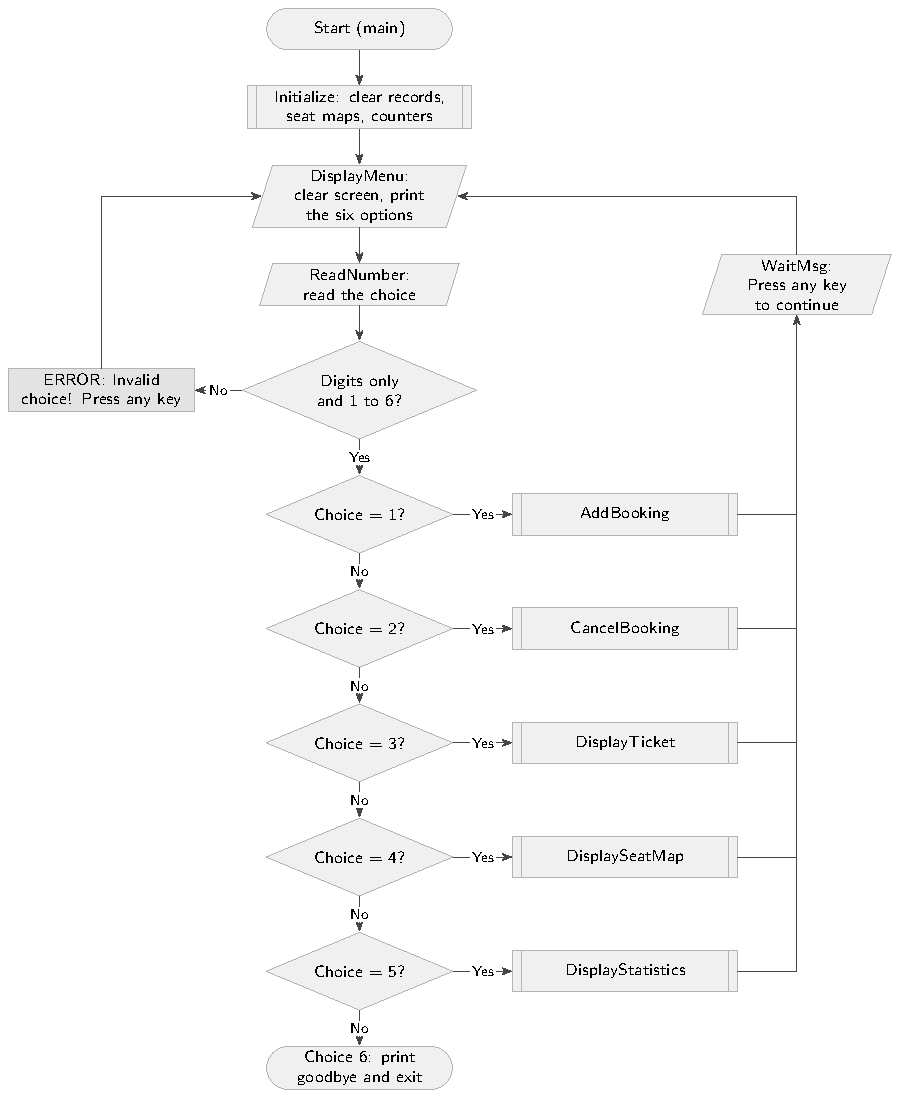
\includegraphics[height=0.6\textheight,width=0.95\textwidth,keepaspectratio]{diagrams/main-flow.pdf}
\captionof{figure}{Main program flowchart: initialisation, menu loop, invalid choice handling and dispatch to all six options.}
\label{fig:main-flow}
\end{minipage}

\bigskip
The menu loop is a condition-controlled loop built from \texttt{CMP} and \texttt{JMP}, because the number of operations a user performs is not known in advance. The dispatch is an IF-ELSE chain: the choice is compared with 1, 2, 3, 4 and 5 in turn, and anything left is the exit choice.

\section{Book Ticket Procedure Flowchart}

\begin{minipage}{\textwidth}
\texttt{AddBooking} collects the five stored fields into a 37-byte staging record, \texttt{newRec}, and copies it into the booking array only after every field has passed validation. A booking that is abandoned part way through (a full movie) therefore never leaves a half-written record in the array. The flow is shown in two parts: capacity, name, booking ID and movie (Figure~\ref{fig:book-a}), then seat, category, price and storage (Figure~\ref{fig:book-b}).

\medskip
\centering
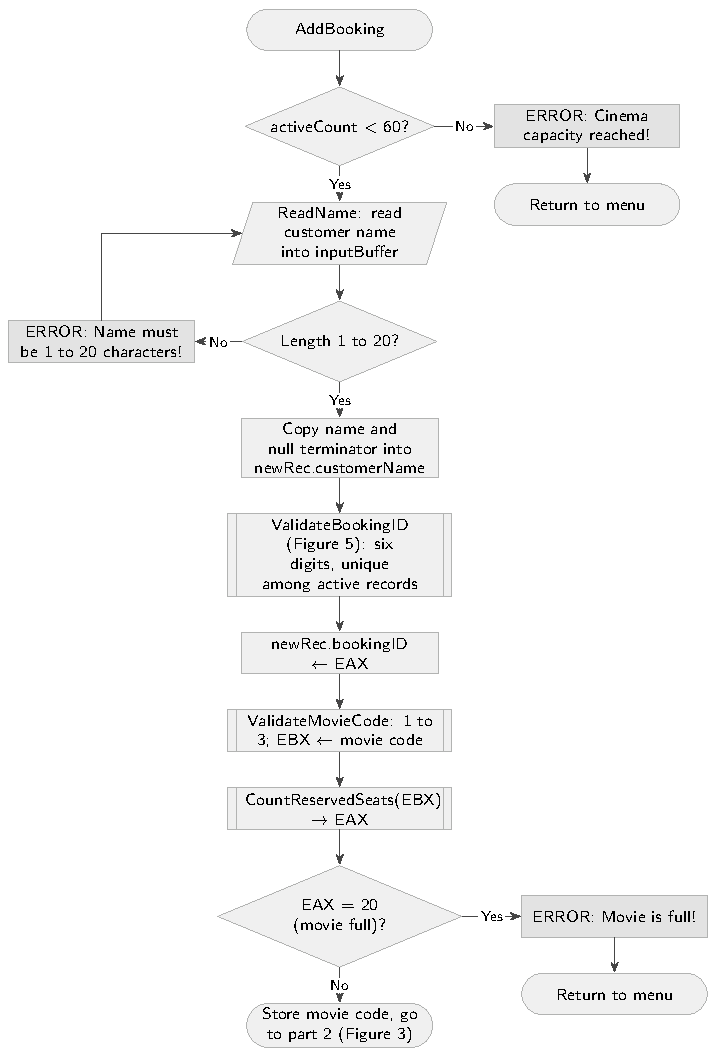
\includegraphics[height=0.62\textheight,width=0.95\textwidth,keepaspectratio]{diagrams/book-ticket-a.pdf}
\captionof{figure}{Book Ticket, part 1: capacity check, customer name, booking ID and movie code with the full-movie check.}
\label{fig:book-a}
\end{minipage}

\begin{figure}[H]
\centering
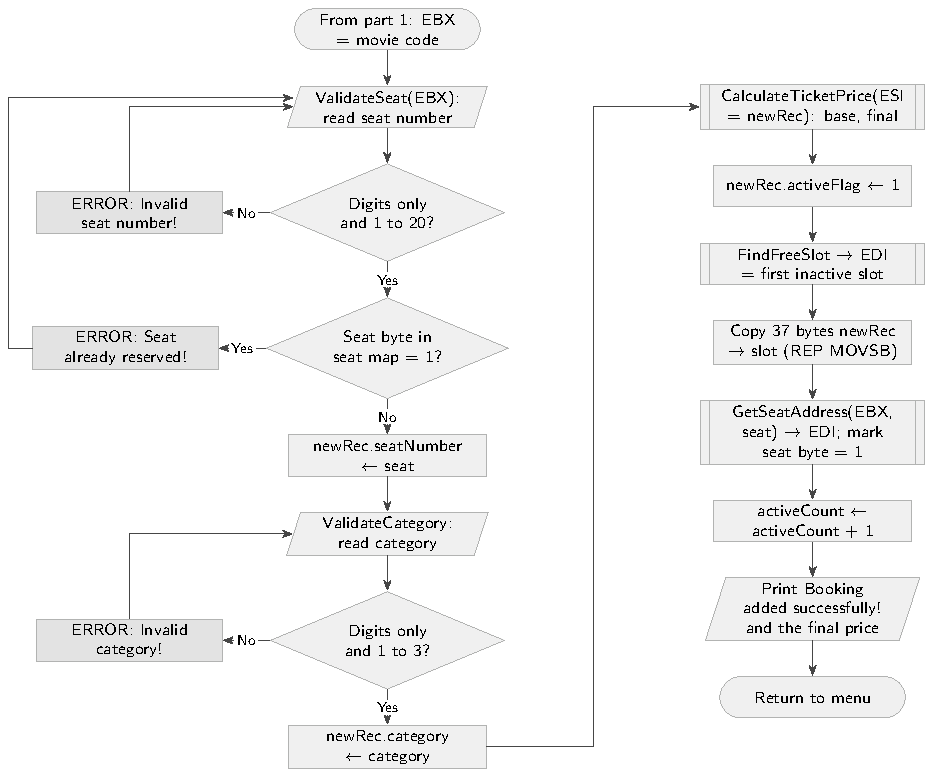
\includegraphics[width=0.98\textwidth]{diagrams/book-ticket-b.pdf}
\caption{Book Ticket, part 2: seat and category validation, price calculation and writing the record.}
\label{fig:book-b}
\end{figure}

Three design decisions are visible in the two parts:

\begin{itemize}
\item \textbf{Two different kinds of error.} An invalid value (a bad name, ID, seat or category) is re-read at once, because the user can correct it. A capacity problem (60 active bookings, or a movie with all 20 seats taken) cannot be fixed by typing again, so it shows its error and returns to the menu.
\item \textbf{The full-movie check comes before the seat prompt.} Checking a movie as soon as it is chosen stops the user being asked for a seat that can never be valid.
\item \textbf{The free slot is found last.} \texttt{FindFreeSlot} cannot fail at that point, because the capacity check at the start already proved that fewer than 60 records are active. A slot freed by a cancellation is reused, since the search looks for the first record whose active flag is 0.
\end{itemize}

\section{Validation and Search Flowcharts}

All numeric input passes through one procedure, \texttt{ReadNumber}, so the digit check required by Section 2.1 of the Phase 1 document is written once and used by every prompt. The Irvine32 \texttt{ReadInt} routine is not used: it accepts a leading sign and prints its own error message, while the brief requires specific error messages for each field.

\begin{minipage}{\textwidth}
\texttt{ReadNumber} reads the whole line as text, rejects an empty line or a line longer than six characters, then converts it one character at a time. Any character outside \texttt{`0'} to \texttt{`9'} makes the whole input invalid. Limiting the input to six digits also means the value can never overflow a doubleword. The procedure reports success or failure in the carry flag, and the caller then applies its own range check and error message.

\medskip
\centering
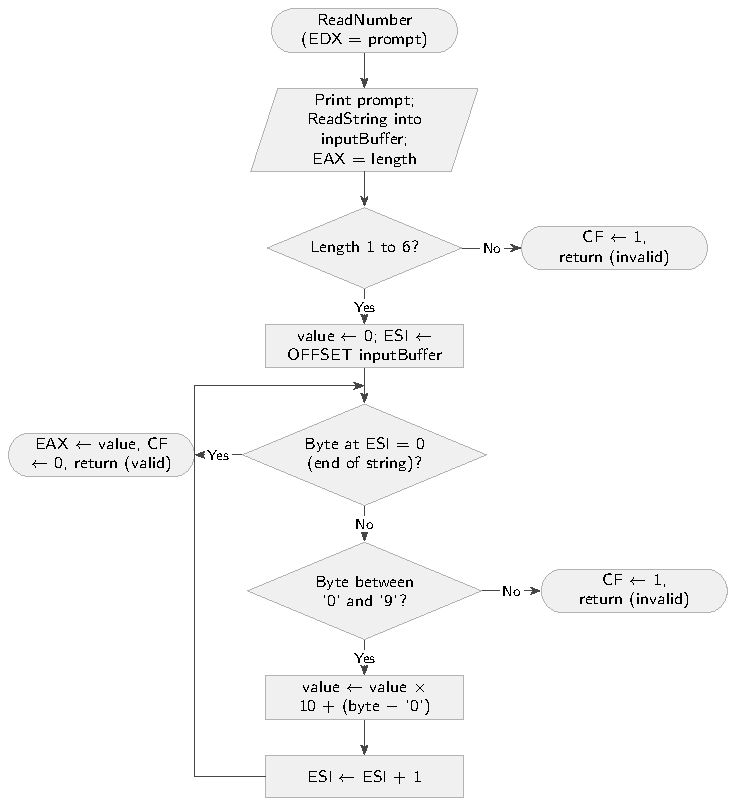
\includegraphics[height=0.55\textheight,width=0.8\textwidth,keepaspectratio]{diagrams/read-number.pdf}
\captionof{figure}{Numeric input validation in \texttt{ReadNumber}: length check, digit check and conversion to an integer.}
\label{fig:read-number}
\end{minipage}

\begin{figure}[H]
\centering
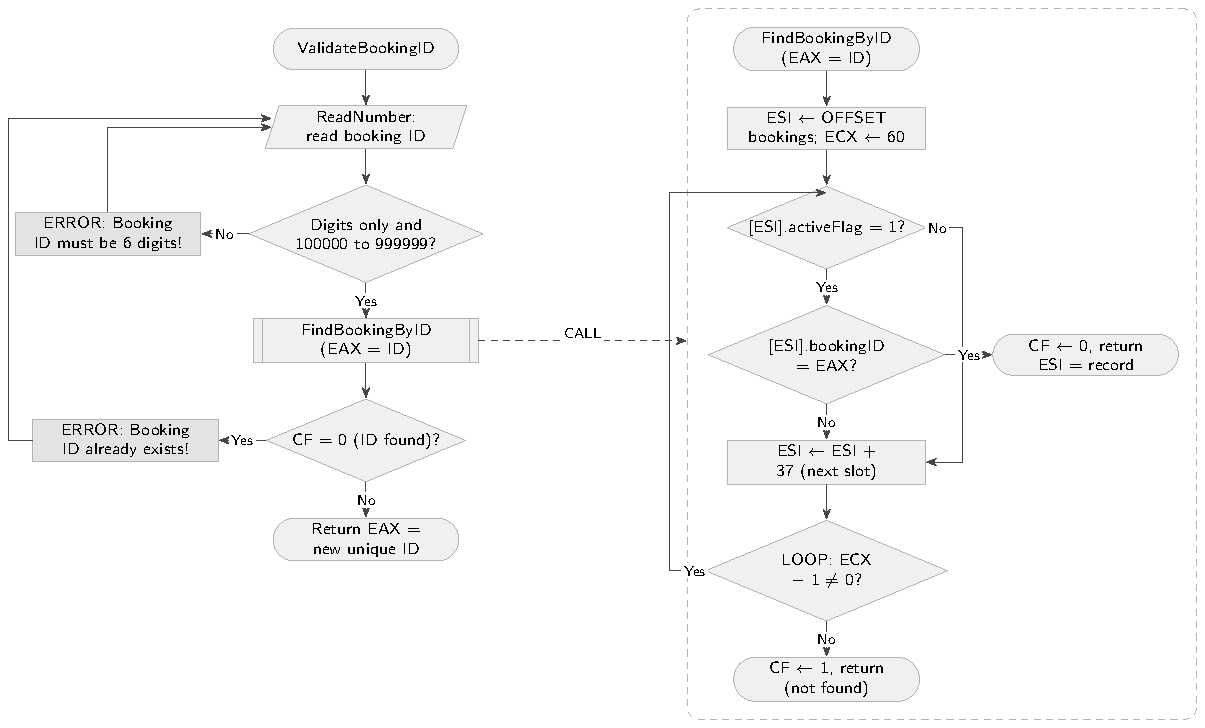
\includegraphics[width=0.98\textwidth]{diagrams/validate-id.pdf}
\caption{Booking ID uniqueness: \texttt{ValidateBookingID} calls the linear search \texttt{FindBookingByID} over the 60 record slots.}
\label{fig:validate-id}
\end{figure}

\texttt{FindBookingByID} is a linear search. It visits all 60 slots with the \texttt{LOOP} instruction, and a slot only matches when its active flag is 1 \textbf{and} its booking ID equals the one wanted. These two tests form a nested condition. Testing the flag first is what makes a cancelled record invisible: its ID can be used again by a new booking, as stated in Assumption 5 of the Phase 1 document. The same search is used by \texttt{CancelBooking} and \texttt{DisplayTicket}, where finding no match produces \texttt{ERROR: Booking ID not found!}.

\begin{figure}[H]
\centering
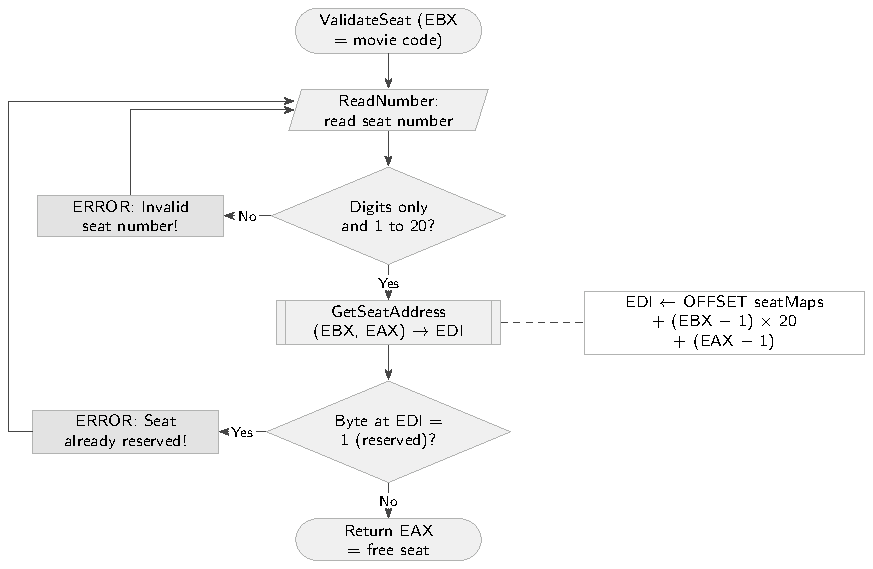
\includegraphics[width=0.85\textwidth]{diagrams/validate-seat.pdf}
\caption{Seat availability in \texttt{ValidateSeat}: range check, then a direct look-up in the seat map of the chosen movie.}
\label{fig:validate-seat}
\end{figure}

Seat availability needs no search at all. The seat map holds one byte per seat, so the byte for a given movie and seat is found directly from its address, as shown beside the flowchart. Because the seat map belongs to one movie, seat 5 of Movie A and seat 5 of Movie B are separate bytes, as required by Assumption 1 of the Phase 1 document.

\section{Cancellation, Display and Statistics Flowcharts}

The remaining menu options each have their own flowchart below, so every procedure called from \texttt{main} is covered by a flowchart as well as by pseudocode. They reuse the procedures already shown: \texttt{ReadBookingID} and \texttt{FindBookingByID} (Figure~\ref{fig:validate-id}), \texttt{ValidateMovieCode} and \texttt{GetSeatAddress} (Figure~\ref{fig:validate-seat}).

\begin{minipage}{\textwidth}
\texttt{CancelBooking} never deletes a record. It clears the active flag, which frees the slot for \texttt{FindFreeSlot} and hides the record from every search and report, then releases the seat byte so the same seat can be sold again in the same run.

\medskip
\centering
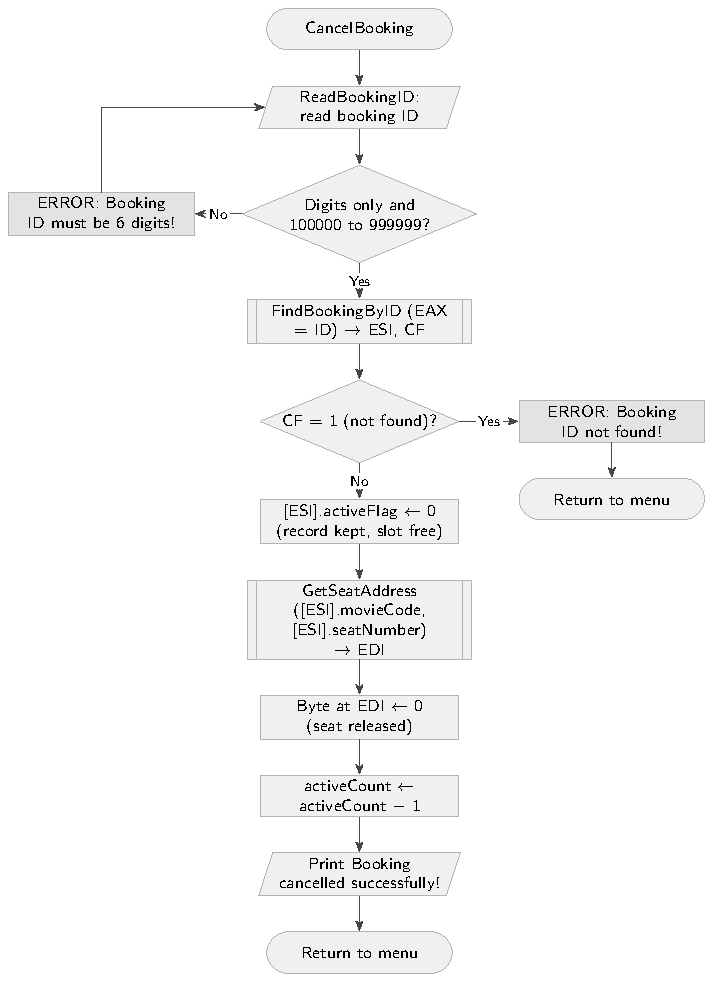
\includegraphics[height=0.62\textheight,width=0.9\textwidth,keepaspectratio]{diagrams/cancel-booking.pdf}
\captionof{figure}{\texttt{CancelBooking}: find the active record, clear its flag, release its seat and update the count.}
\label{fig:cancel}
\end{minipage}

\begin{minipage}{\textwidth}
\texttt{DisplayTicket} uses the same search but only reads the record. The discount is not stored, so it is worked out as base price minus final price while the ticket is printed.

\medskip
\centering
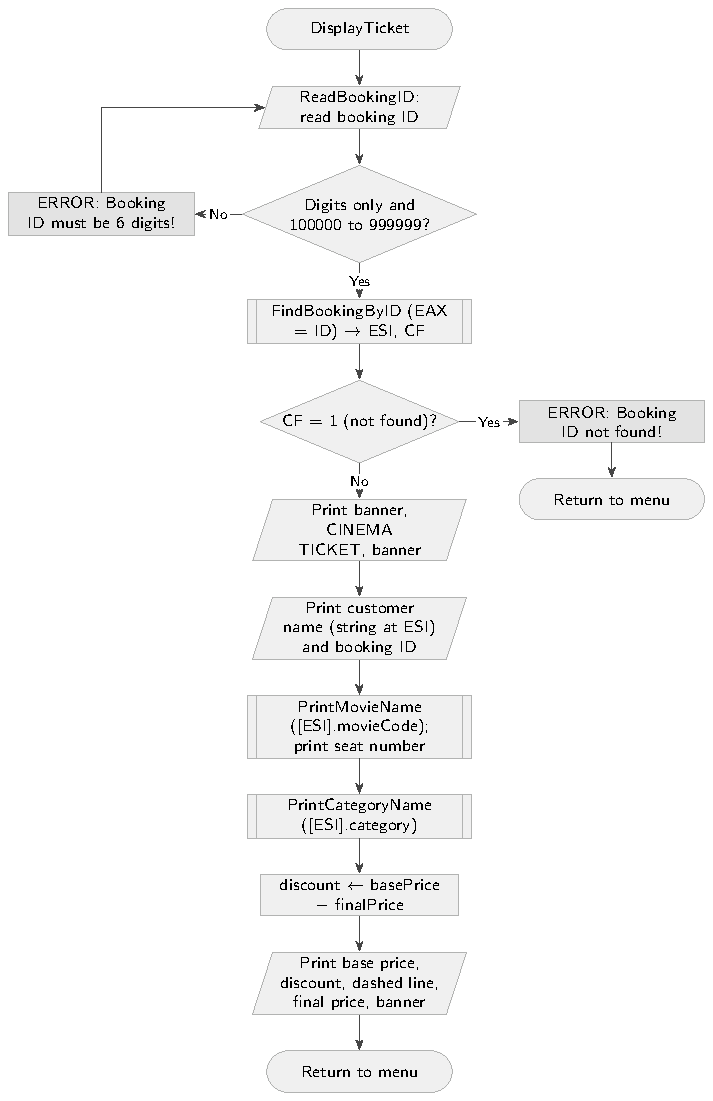
\includegraphics[height=0.62\textheight,width=0.9\textwidth,keepaspectratio]{diagrams/display-ticket.pdf}
\captionof{figure}{\texttt{DisplayTicket}: find the active record and print it in the ticket format of the brief.}
\label{fig:display}
\end{minipage}

\begin{minipage}{\textwidth}
\texttt{DisplaySeatMap} prints the 20 seats as 4 rows of 5 with two nested \texttt{LOOP} instructions. Both use ECX, so the outer count is saved with \texttt{PUSH} before the inner loop and restored with \texttt{POP} after it. A leading zero keeps the seat numbers two digits wide, so the columns line up.

\medskip
\centering
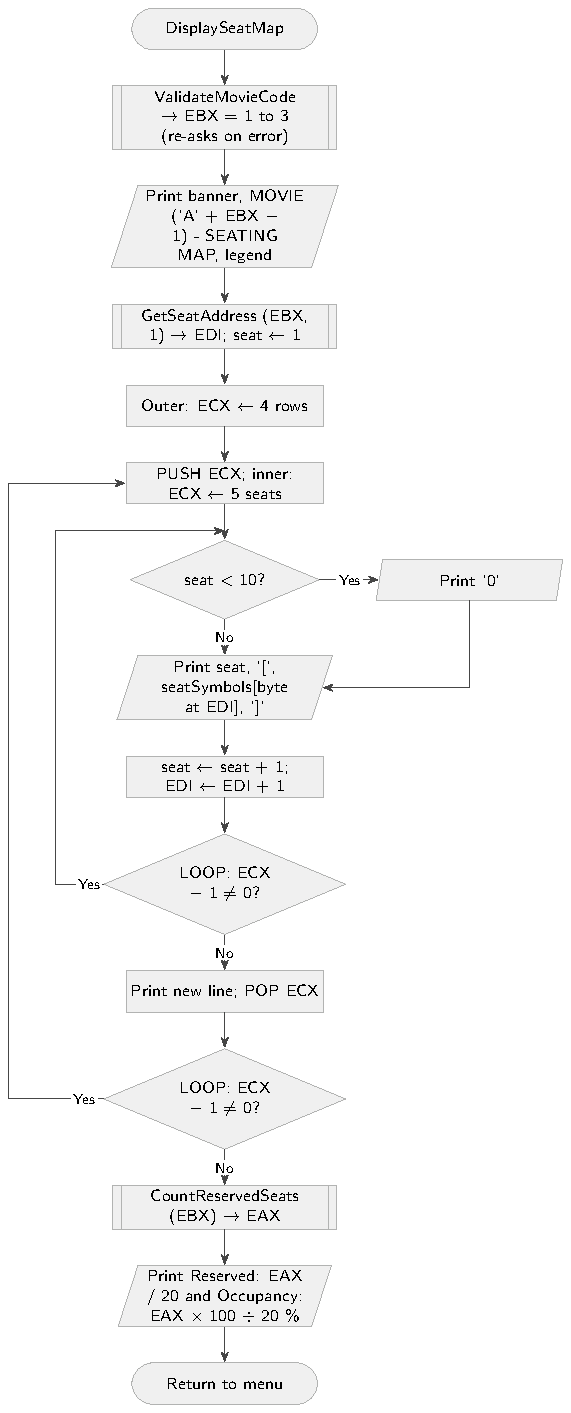
\includegraphics[height=0.7\textheight,width=0.9\textwidth,keepaspectratio]{diagrams/seating-map.pdf}
\captionof{figure}{\texttt{DisplaySeatMap}: nested row and seat loops, then the reserved count and occupancy.}
\label{fig:seatmap}
\end{minipage}

\begin{minipage}{\textwidth}
Statistics are split in two. \texttt{CalculateStatistics} (Figure~\ref{fig:stats-a}) scans the 60 slots and derives every figure, and \texttt{DisplayStatistics} with \texttt{DisplayHistogram} (Figure~\ref{fig:stats-b}) only prints. The check on \texttt{activeCount} before the division stops a divide error when there are no bookings.

\medskip
\centering
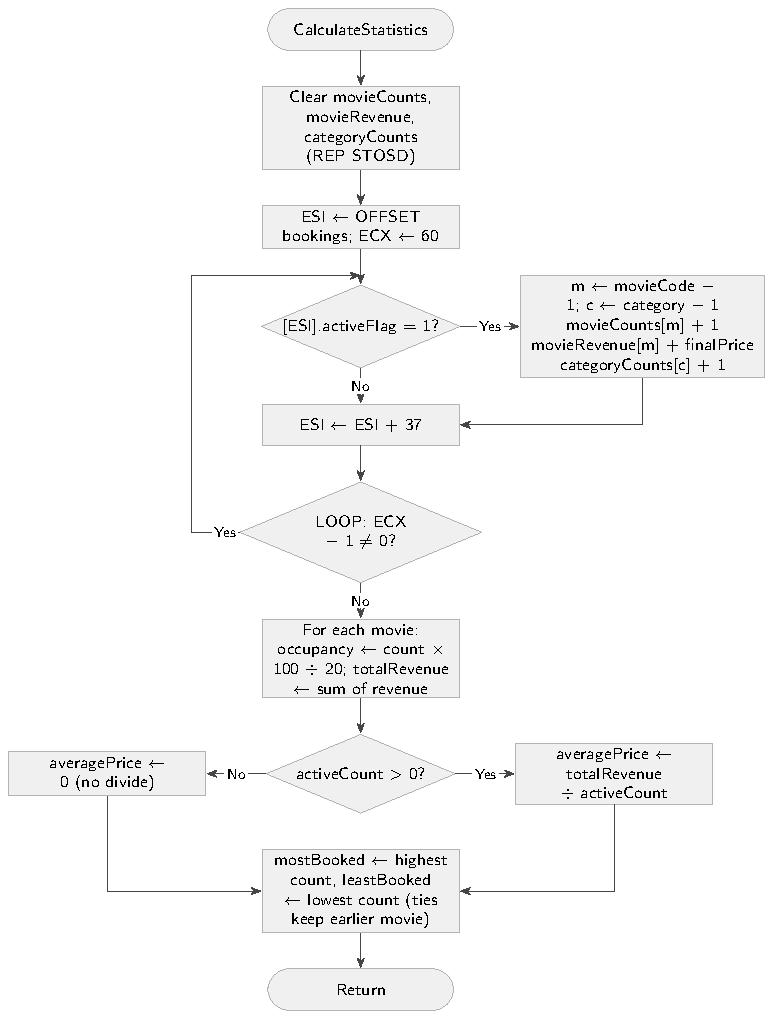
\includegraphics[height=0.62\textheight,width=0.9\textwidth,keepaspectratio]{diagrams/statistics-a.pdf}
\captionof{figure}{\texttt{CalculateStatistics}: scan the active records, then derive occupancy, totals, average and most and least booked.}
\label{fig:stats-a}
\end{minipage}

\begin{figure}[H]
\centering
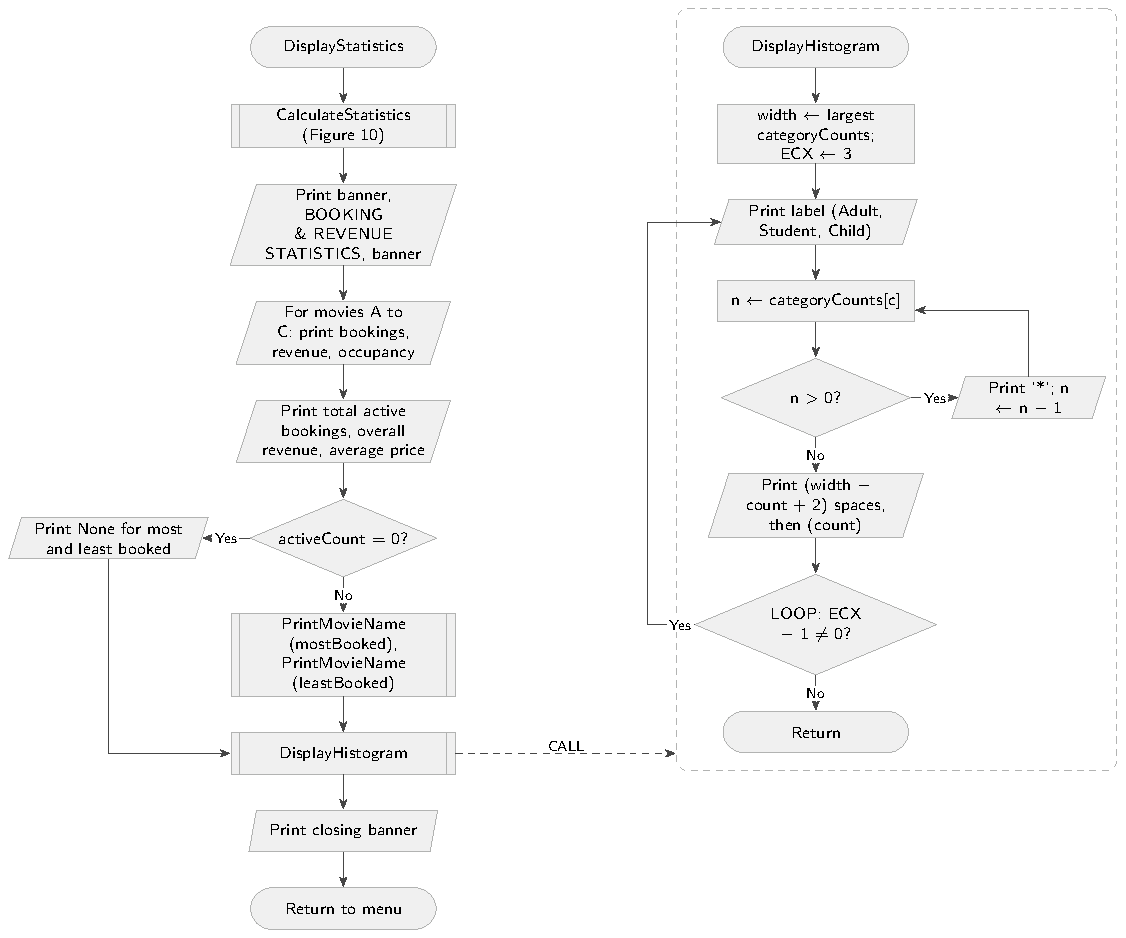
\includegraphics[width=0.98\textwidth]{diagrams/statistics-b.pdf}
\caption{\texttt{DisplayStatistics} and \texttt{DisplayHistogram}: print the report and the category histogram.}
\label{fig:stats-b}
\end{figure}

\section{Pseudocode}

The pseudocode below covers all 24 procedures (the 14 named in the brief and 10 helpers). It uses \texttt{<-} for assignment and the field names of the \texttt{BOOKING} record from Table~\ref{tab:record}. \texttt{[ESI].field} means the field of the record whose address is in ESI. Every procedure saves the registers it uses and restores them before \texttt{RET}, except the registers it returns a result in (Section~\ref{sec:params}).

\subsection{Program control}

\begin{lstlisting}
PROCEDURE main
    CALL Initialize
    WHILE TRUE                                   ; JMP-based loop
        EAX <- CALL DisplayMenu                  ; always 1..6
        IF EAX = 6 THEN EXIT WHILE
        IF EAX = 1 THEN CALL AddBooking
        ELSE IF EAX = 2 THEN CALL CancelBooking
        ELSE IF EAX = 3 THEN CALL DisplayTicket
        ELSE IF EAX = 4 THEN CALL DisplaySeatMap
        ELSE CALL DisplayStatistics
        CALL WaitMsg                             ; "Press any key to continue..."
    END WHILE
    print "Thank you for using CTRMS. Goodbye!"
    exit
END main

PROCEDURE Initialize
    ; bookings .. leastBooked are contiguous (Section 2.3): 2,348 bytes
    CLD                                          ; DF = 0, so REP moves forwards
    EDI <- OFFSET bookings
    ECX <- 2348
    AL  <- 0
    REP STOSB                                    ; every activeFlag and seat byte = 0
END Initialize

PROCEDURE DisplayMenu                            ; returns EAX = 1..6
    WHILE TRUE
        Clrscr
        print the banner and options 1..6
        EAX, CF <- CALL ReadNumber("Enter your choice (1-6): ")
        IF CF = 0 AND EAX >= 1 AND EAX <= 6 THEN RETURN
        print "ERROR: Invalid choice! Please enter 1 to 6."
        CALL WaitMsg
    END WHILE
END DisplayMenu
\end{lstlisting}

\subsection{Input helpers}

\begin{lstlisting}
PROCEDURE ReadNumber                             ; in: EDX = prompt; out: EAX, CF
    print string at EDX
    EAX <- ReadString(inputBuffer, BUF_SIZE)     ; EAX = length
    IF EAX = 0 OR EAX > 6 THEN CF <- 1; RETURN
    value <- 0
    ESI <- OFFSET inputBuffer
    WHILE byte at ESI <> 0                       ; JMP-based loop
        ch <- byte at ESI
        IF ch < '0' OR ch > '9' THEN CF <- 1; RETURN
        value <- value * 10 + (ch - '0')
        ESI <- ESI + 1
    END WHILE
    EAX <- value
    CF  <- 0
END ReadNumber

PROCEDURE ReadName                               ; out: inputBuffer, EAX = length
    WHILE TRUE
        print "Enter customer name (1-20 characters): "
        EAX <- ReadString(inputBuffer, BUF_SIZE)
        IF EAX >= 1 AND EAX <= 20 THEN RETURN
        print "ERROR: Name must be 1 to 20 characters!"
    END WHILE
END ReadName

PROCEDURE ReadBookingID                          ; out: EAX = 100000..999999
    WHILE TRUE
        EAX, CF <- CALL ReadNumber("Enter booking ID (6 digits): ")
        IF CF = 0 AND EAX >= 100000 AND EAX <= 999999 THEN RETURN
        print "ERROR: Booking ID must be 6 digits (100000-999999)!"
    END WHILE
END ReadBookingID
\end{lstlisting}

\subsection{Booking and validation}

\begin{lstlisting}
PROCEDURE AddBooking
    IF activeCount >= 60 THEN
        print "ERROR: Cinema capacity reached!"; RETURN
    EAX <- CALL ReadName
    copy EAX + 1 bytes (name and null) from inputBuffer to newRec.customerName
    newRec.bookingID <- CALL ValidateBookingID
    EBX <- CALL ValidateMovieCode
    IF CALL CountReservedSeats(EBX) = 20 THEN
        print "ERROR: Movie is full!"; RETURN
    newRec.movieCode  <- BL
    newRec.seatNumber <- CALL ValidateSeat(EBX)
    newRec.category   <- CALL ValidateCategory
    ESI <- OFFSET newRec
    CALL CalculateTicketPrice(ESI)               ; fills basePrice and finalPrice
    newRec.activeFlag <- 1
    EDI <- CALL FindFreeSlot                     ; cannot fail: activeCount < 60
    copy 37 bytes from ESI to EDI (REP MOVSB)
    EDI <- CALL GetSeatAddress(EBX, newRec.seatNumber)
    byte at EDI <- 1                             ; seat reserved
    activeCount <- activeCount + 1
    print "Booking added successfully!"
    print "Final Ticket Price: ", newRec.finalPrice, " JOD"
END AddBooking

PROCEDURE ValidateBookingID                      ; out: EAX = unique ID
    WHILE TRUE
        EAX <- CALL ReadBookingID
        CALL FindBookingByID(EAX)
        IF CF = 1 THEN RETURN                    ; no active record has this ID
        print "ERROR: Booking ID already exists!"
    END WHILE
END ValidateBookingID

PROCEDURE ValidateMovieCode                      ; out: EAX = 1..3
    WHILE TRUE
        EAX, CF <- CALL ReadNumber("Enter movie code (1=A, 2=B, 3=C): ")
        IF CF = 0 AND EAX >= 1 AND EAX <= 3 THEN RETURN
        print "ERROR: Invalid movie code! Please enter 1 to 3."
    END WHILE
END ValidateMovieCode

PROCEDURE ValidateSeat                           ; in: EBX = movie; out: EAX = seat
    WHILE TRUE
        EAX, CF <- CALL ReadNumber("Enter seat number (1-20): ")
        IF CF = 1 OR EAX < 1 OR EAX > 20 THEN
            print "ERROR: Invalid seat number! Please enter 1 to 20."
        ELSE
            EDI <- CALL GetSeatAddress(EBX, EAX)
            IF byte at EDI = 1 THEN              ; nested IF-ELSE
                print "ERROR: Seat already reserved!"
            ELSE
                RETURN
            END IF
        END IF
    END WHILE
END ValidateSeat

PROCEDURE ValidateCategory                       ; out: EAX = 1..3
    WHILE TRUE
        EAX, CF <- CALL ReadNumber("Enter category (1=Adult, 2=Student, 3=Child): ")
        IF CF = 0 AND EAX >= 1 AND EAX <= 3 THEN RETURN
        print "ERROR: Invalid category! Please enter 1 to 3."
    END WHILE
END ValidateCategory

PROCEDURE CalculateTicketPrice                   ; in: ESI = record; out: EAX = final
    EBX <- [ESI].movieCode - 1                   ; index 0..2
    base <- basePriceTable[EBX * 4]              ; 8, 7 or 6 JOD
    EBX <- [ESI].category - 1
    EAX <- base - discountTable[EBX * 4]         ; minus 0, 1 or 2 JOD
    [ESI].basePrice  <- base
    [ESI].finalPrice <- EAX
END CalculateTicketPrice
\end{lstlisting}

Table~\ref{tab:prices} lists the nine results \texttt{CalculateTicketPrice} must produce. Only \texttt{SUB} is needed, so the calculation is pure integer arithmetic.

\begin{table}[H]
\centering
\tablefont
\caption{Price results for every movie and category combination (JOD)}
\label{tab:prices}
\begin{tabular}{|l|c|c|c|}
\hline
\textbf{Movie (base price)} & \textbf{Adult ($-$0)} & \textbf{Student ($-$1)} & \textbf{Child ($-$2)} \\
\hline
Movie A (8) & 8 & 7 & 6 \\
\hline
Movie B (7) & 7 & 6 & 5 \\
\hline
Movie C (6) & 6 & 5 & 4 \\
\hline
\end{tabular}
\end{table}

\subsection{Searching, seats and cancellation}

\begin{lstlisting}
PROCEDURE FindBookingByID                        ; in: EAX = ID; out: ESI, CF
    ESI <- OFFSET bookings
    ECX <- 60
    REPEAT                                       ; LOOP instruction
        IF [ESI].activeFlag = 1 THEN
            IF [ESI].bookingID = EAX THEN CF <- 0; RETURN
        END IF
        ESI <- ESI + 37
    UNTIL --ECX = 0
    CF <- 1                                      ; not found
END FindBookingByID

PROCEDURE FindFreeSlot                           ; out: EDI, CF
    EDI <- OFFSET bookings
    ECX <- 60
    REPEAT                                       ; LOOP instruction
        IF [EDI].activeFlag = 0 THEN CF <- 0; RETURN
        EDI <- EDI + 37
    UNTIL --ECX = 0
    CF <- 1                                      ; every slot is active
END FindFreeSlot

PROCEDURE GetSeatAddress                         ; in: EBX = movie, EAX = seat; out: EDI
    EDI <- OFFSET seatMaps + (EBX - 1) * 20 + (EAX - 1)
END GetSeatAddress

PROCEDURE CountReservedSeats                     ; in: EBX = movie; out: EAX = 0..20
    EDI <- CALL GetSeatAddress(EBX, 1)
    EAX <- 0
    ECX <- 20
    REPEAT                                       ; LOOP instruction
        IF byte at EDI = 1 THEN EAX <- EAX + 1
        EDI <- EDI + 1
    UNTIL --ECX = 0
END CountReservedSeats

PROCEDURE CancelBooking
    EAX <- CALL ReadBookingID
    CALL FindBookingByID(EAX)
    IF CF = 1 THEN
        print "ERROR: Booking ID not found!"
    ELSE
        [ESI].activeFlag <- 0                    ; record stays, slot is free
        EDI <- CALL GetSeatAddress([ESI].movieCode, [ESI].seatNumber)
        byte at EDI <- 0                         ; seat released
        activeCount <- activeCount - 1
        print "Booking cancelled successfully!"
    END IF
END CancelBooking
\end{lstlisting}

\subsection{Display procedures}

\begin{lstlisting}
PROCEDURE DisplayTicket
    EAX <- CALL ReadBookingID
    CALL FindBookingByID(EAX)
    IF CF = 1 THEN
        print "ERROR: Booking ID not found!"
    ELSE
        print banner line, "CINEMA TICKET", banner line
        print "Customer Name: ", string at ESI
        print "Booking ID: ", [ESI].bookingID
        print "Movie: ";            CALL PrintMovieName([ESI].movieCode)
        print "Seat Number: ", [ESI].seatNumber
        print "Ticket Category: ";  CALL PrintCategoryName([ESI].category)
        print "Base Price: ", [ESI].basePrice, " JOD"
        print "Discount: ", [ESI].basePrice - [ESI].finalPrice, " JOD"
        print dashed line
        print "Final Ticket Price: ", [ESI].finalPrice, " JOD"
        print banner line
    END IF
END DisplayTicket

PROCEDURE DisplaySeatMap
    EBX <- CALL ValidateMovieCode
    print banner, "MOVIE ", character ('A' + EBX - 1), " - SEATING MAP", banner
    print "Legend: [O] Available   [X] Reserved"
    EDI <- CALL GetSeatAddress(EBX, 1)
    seat <- 1
    FOR row <- 1 TO 4                            ; outer LOOP, ECX saved with PUSH
        FOR col <- 1 TO 5                        ; inner LOOP
            IF seat < 10 THEN print '0'          ; two-digit seat numbers
            print seat, '[', seatSymbols[byte at EDI], ']', ' '
            seat <- seat + 1
            EDI  <- EDI + 1
        END FOR
        print new line
    END FOR
    EAX <- CALL CountReservedSeats(EBX)
    print "Reserved: ", EAX, " / 20"
    print "Occupancy: ", (EAX * 100) / 20, "%"   ; MUL then DIV, integer only
END DisplaySeatMap
\end{lstlisting}

\subsection{Statistics}

\begin{lstlisting}
PROCEDURE CalculateStatistics
    clear movieCounts, movieRevenue and categoryCounts (9 DWORDs, REP STOSD)
    ESI <- OFFSET bookings
    ECX <- 60
    REPEAT                                       ; LOOP instruction
        IF [ESI].activeFlag = 1 THEN             ; cancelled records are skipped
            m <- [ESI].movieCode - 1
            c <- [ESI].category  - 1
            movieCounts[m]    <- movieCounts[m] + 1
            movieRevenue[m]   <- movieRevenue[m] + [ESI].finalPrice
            categoryCounts[c] <- categoryCounts[c] + 1
        END IF
        ESI <- ESI + 37
    UNTIL --ECX = 0
    totalRevenue <- 0
    FOR m <- 0 TO 2
        movieOccupancy[m] <- movieCounts[m] * 100 / 20
        totalRevenue      <- totalRevenue + movieRevenue[m]
    END FOR
    IF activeCount > 0 THEN                      ; avoids a divide error
        averagePrice <- totalRevenue / activeCount
    ELSE
        averagePrice <- 0
    END IF
    mostBooked <- 1;  leastBooked <- 1
    FOR m <- 2 TO 3                              ; ties keep the earlier movie
        IF movieCounts[m-1] > movieCounts[mostBooked-1]  THEN mostBooked  <- m
        IF movieCounts[m-1] < movieCounts[leastBooked-1] THEN leastBooked <- m
    END FOR
END CalculateStatistics

PROCEDURE DisplayStatistics
    CALL CalculateStatistics
    print banner, "BOOKING & REVENUE STATISTICS", banner
    FOR m <- 1 TO 3
        CALL PrintMovieName(m)
        print ": ", movieCounts[m-1], " bookings   Revenue: ", movieRevenue[m-1],
              " JOD   Occupancy: ", movieOccupancy[m-1], "%"
    END FOR
    print dashed line
    print "Total Active Bookings: ", activeCount
    print "Overall Revenue: ", totalRevenue, " JOD"
    print "Average Ticket Price: ", averagePrice, " JOD"
    IF activeCount = 0 THEN
        print "Most Booked Movie: None";  print "Least Booked Movie: None"
    ELSE
        print "Most Booked Movie: ";  CALL PrintMovieName(mostBooked)
        print "Least Booked Movie: "; CALL PrintMovieName(leastBooked)
    END IF
    CALL DisplayHistogram
    print banner
END DisplayStatistics

PROCEDURE DisplayHistogram
    print "TICKET CATEGORY DISTRIBUTION:"
    width <- largest of categoryCounts[0..2]
    FOR c <- 0 TO 2                              ; outer LOOP
        print histogram label c                  ; "Adult   : " etc.
        n <- categoryCounts[c]
        WHILE n > 0                              ; JMP-based: n may be 0
            print '*';  n <- n - 1
        END WHILE
        print (width - categoryCounts[c] + 2) spaces
        print "(", categoryCounts[c], ")"
    END FOR
END DisplayHistogram

PROCEDURE PrintMovieName                         ; in: EAX = movie code 1..3
    EDX <- movieNames[(EAX - 1) * 4];  WriteString
END PrintMovieName

PROCEDURE PrintCategoryName                      ; in: EAX = category 1..3
    EDX <- categoryNames[(EAX - 1) * 4];  WriteString
END PrintCategoryName
\end{lstlisting}

The histogram pads every row to the same width before the count, so the counts line up as in the brief (\texttt{********~~(8)}, \texttt{*****~~~~~(5)}). The star loop is a \texttt{JMP}-based while loop rather than \texttt{LOOP}, because a category may have no bookings: \texttt{LOOP} with ECX = 0 would decrement ECX to FFFFFFFFh and run more than four billion times.

% ── Chapter 2: Data Structure Design ────────────────────────────────────────

\printchaptertitle{Data Structure Design}

\section{Booking Record Structure}

Each booking is one fixed-size record of 37 bytes. Table~\ref{tab:record} defines every field. The layout is the one in Table 4 of the Phase 1 document: a 21-byte name field holds the longest valid name (20 characters) plus its null terminator. The sample in Appendix C of the brief uses a 20-byte name field, which would leave no room for the terminator after a 20-character name. Every field after the name is therefore one byte further on than in the sample, and the record is 37 bytes rather than 36.

\begin{table}[H]
\centering
\tablefont
\caption{Booking record structure (BOOKING, 37 bytes)}
\label{tab:record}
\begin{tabular}{|c|c|L{0.17\linewidth}|L{0.12\linewidth}|L{0.44\linewidth}|}
\hline
\textbf{Offset} & \textbf{Size} & \textbf{Field} & \textbf{Type} & \textbf{Description} \\
\hline
0 & 21 & customerName & BYTE $\times$ 21 & Customer name, 1 to 20 ASCII characters followed by a null byte \\
\hline
21 & 4 & bookingID & DWORD & Six-digit booking ID, 100000 to 999999, unique among active records \\
\hline
25 & 1 & movieCode & BYTE & 1 = Movie A, 2 = Movie B, 3 = Movie C \\
\hline
26 & 1 & seatNumber & BYTE & Seat 1 to 20 within the chosen movie \\
\hline
27 & 1 & category & BYTE & 1 = Adult, 2 = Student, 3 = Child \\
\hline
28 & 1 & activeFlag & BYTE & 1 = active booking, 0 = cancelled or never used \\
\hline
29 & 4 & basePrice & DWORD & Base price of the movie in JOD (8, 7 or 6) \\
\hline
33 & 4 & finalPrice & DWORD & Base price minus the category discount, in JOD (4 to 8) \\
\hline
\multicolumn{2}{|c|}{\textbf{37}} & \multicolumn{3}{l|}{\textbf{Total record size, SIZEOF BOOKING}} \\
\hline
\end{tabular}
\end{table}

\begin{figure}[H]
\centering
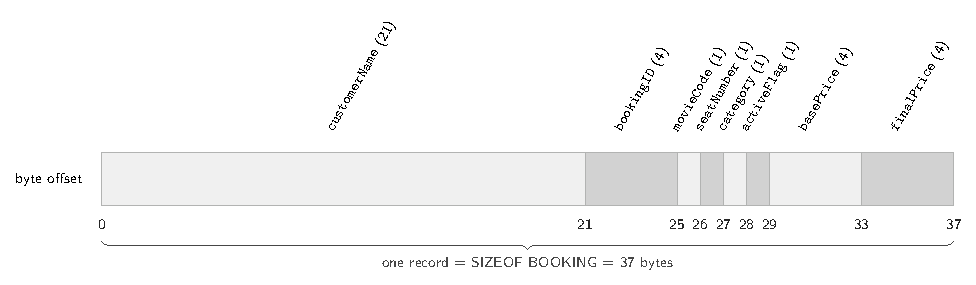
\includegraphics[width=0.98\textwidth]{diagrams/record-layout.pdf}
\caption{Byte layout of one booking record, drawn to scale.}
\label{fig:record}
\end{figure}

The discount is not stored. It is always \texttt{basePrice} $-$ \texttt{finalPrice}, so \texttt{DisplayTicket} works it out with one \texttt{SUB} when it prints the ticket.

\subsection*{MASM definition}

The record is declared as a MASM \texttt{STRUCT}. MASM packs structure fields with no padding unless an alignment is requested, so \texttt{SIZEOF BOOKING} is exactly 37 and each field can be reached by name instead of by a hard-coded number:

\begin{lstlisting}
BOOKING STRUCT                       ; offset  size
    customerName BYTE 21 DUP(0)      ;   0      21   20 characters + null
    bookingID    DWORD 0             ;  21       4
    movieCode    BYTE 0              ;  25       1
    seatNumber   BYTE 0              ;  26       1
    category     BYTE 0              ;  27       1
    activeFlag   BYTE 0              ;  28       1
    basePrice    DWORD 0             ;  29       4
    finalPrice   DWORD 0             ;  33       4
BOOKING ENDS                         ; SIZEOF BOOKING = 37
\end{lstlisting}

\subsection*{Reaching a record by index and offset}

The 60 records are stored back to back in the array \texttt{bookings}. Record $i$ (0 to 59) starts at
\[
\texttt{OFFSET bookings} + i \times 37
\]
and a field of that record is at that address plus the field offset. For example, the booking ID of record 5 is at \texttt{bookings} + 5 $\times$ 37 + 21 = \texttt{bookings} + 206. In practice the procedures never multiply: a scan starts with ESI at \texttt{OFFSET bookings} and adds 37 to move to the next record, then reads a field through the structure name:

\begin{lstlisting}
    mov  esi, OFFSET bookings
    mov  ecx, MAX_BOOKINGS
scan:
    cmp  (BOOKING PTR [esi]).activeFlag, 1    ; byte at [esi + 28]
    jne  next
    cmp  (BOOKING PTR [esi]).bookingID, eax   ; dword at [esi + 21]
    je   found
next:
    add  esi, SIZEOF BOOKING                  ; esi + 37
    loop scan
\end{lstlisting}

The three doubleword fields start at offsets 21, 29 and 33, and records start at multiples of 37, so these fields are not aligned on 4-byte boundaries. IA-32 processors read unaligned doublewords correctly in protected mode, at the cost of a few extra cycles. That cost is negligible for 60 records, and keeping the field order of Phase 1 and the brief keeps the record easy to explain and check.

\section{Array Design}

The program uses four kinds of array: the booking array, the seat maps, the statistics arrays and a set of constant look-up tables. Figure~\ref{fig:arrays} shows the first three, and Table~\ref{tab:arrays} lists every array with its element type and the formula that reaches an element.

\begin{figure}[H]
\centering
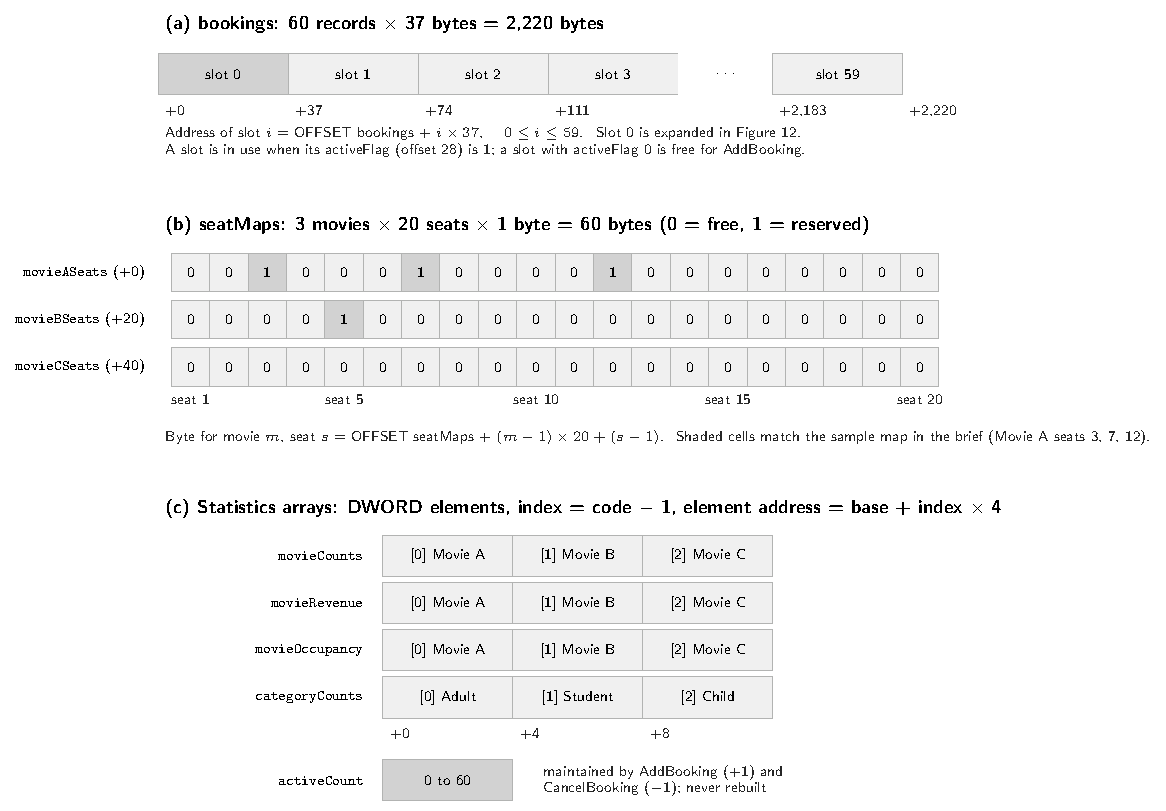
\includegraphics[width=0.98\textwidth]{diagrams/array-design.pdf}
\caption{Array design: the booking array, the three seat maps and the statistics arrays.}
\label{fig:arrays}
\end{figure}

\begin{table}[H]
\centering
\tablefont
\caption{Arrays and how each element is reached}
\label{tab:arrays}
\begin{tabular}{|L{0.19\linewidth}|L{0.13\linewidth}|c|L{0.27\linewidth}|L{0.2\linewidth}|}
\hline
\textbf{Array} & \textbf{Element} & \textbf{Count} & \textbf{Element address} & \textbf{Values} \\
\hline
bookings & BOOKING (37 B) & 60 & bookings + $i \times 37$, $i$ = 0..59 & Record; activeFlag 1 = in use \\
\hline
seatMaps (movieASeats, movieBSeats, movieCSeats) & BYTE & 3 $\times$ 20 & seatMaps + $(m-1)\times 20 + (s-1)$ & 0 = free, 1 = reserved \\
\hline
movieCounts & DWORD & 3 & movieCounts + $(m-1)\times 4$ & Active bookings per movie, 0..20 \\
\hline
movieRevenue & DWORD & 3 & movieRevenue + $(m-1)\times 4$ & JOD per movie, 0..160 \\
\hline
movieOccupancy & DWORD & 3 & movieOccupancy + $(m-1)\times 4$ & Percent per movie, 0..100 \\
\hline
categoryCounts & DWORD & 3 & categoryCounts + $(c-1)\times 4$ & Adult, Student, Child counts \\
\hline
basePriceTable & DWORD & 3 & basePriceTable + $(m-1)\times 4$ & 8, 7, 6 \\
\hline
discountTable & DWORD & 3 & discountTable + $(c-1)\times 4$ & 0, 1, 2 \\
\hline
movieNames, categoryNames & DWORD (address) & 3 each & table + $(\text{code}-1)\times 4$ & Address of the name string \\
\hline
seatSymbols & BYTE (character) & 2 & seatSymbols + seat byte & `O' (free), `X' (reserved) \\
\hline
\end{tabular}
\end{table}

\subsection*{Seat maps}

The brief suggests three separate arrays, \texttt{movieASeats}, \texttt{movieBSeats} and \texttt{movieCSeats}. They are kept, but declared one after another under a single label \texttt{seatMaps}. The three 20-byte arrays then form one 60-byte block, and \texttt{GetSeatAddress} can reach any seat of any movie with one formula instead of a three-way branch. The seat byte also indexes \texttt{seatSymbols}, so the seating map prints \texttt{O} or \texttt{X} without an IF-ELSE.

\subsection*{Statistics arrays}

\texttt{movieCounts}, \texttt{movieRevenue} and \texttt{categoryCounts} are the arrays suggested in Appendix C of the brief. \texttt{movieOccupancy} and the four single values \texttt{totalRevenue}, \texttt{averagePrice}, \texttt{mostBooked} and \texttt{leastBooked} are added so that \texttt{CalculateStatistics} produces every figure in the report and \texttt{DisplayStatistics} only prints. All of them are rebuilt from the records each time option 5 is chosen (Section 2.3.6 of the Phase 1 document), so cancelled records can never leave stale totals behind.

\texttt{activeCount} is the one counter that is kept up to date instead of being rebuilt: \texttt{AddBooking} adds 1 and \texttt{CancelBooking} subtracts 1. This lets the capacity check at the start of every booking run without scanning 60 records.

All counters are DWORDs, even where a byte would hold the value (at most 60 bookings, 160 JOD per movie, 480 JOD in total). A DWORD can be loaded straight into EAX for \texttt{WriteDec}, \texttt{MUL} and \texttt{DIV}, with no \texttt{MOVZX} needed.

\section{Memory Map}

Figure~\ref{fig:memory} shows the data segment in the order the variables will be declared. MASM places variables in declaration order, so each offset is the sum of the sizes above it. The first group matches Table 4 of the Phase 1 document exactly: 2,220 + 60 + 12 + 12 + 12 + 4 = \textbf{2,320 bytes}. The groups below it are new in this phase: the derived statistics, the staging record and input buffer used while a booking is entered, and the constant tables.

\begin{figure}[H]
\centering
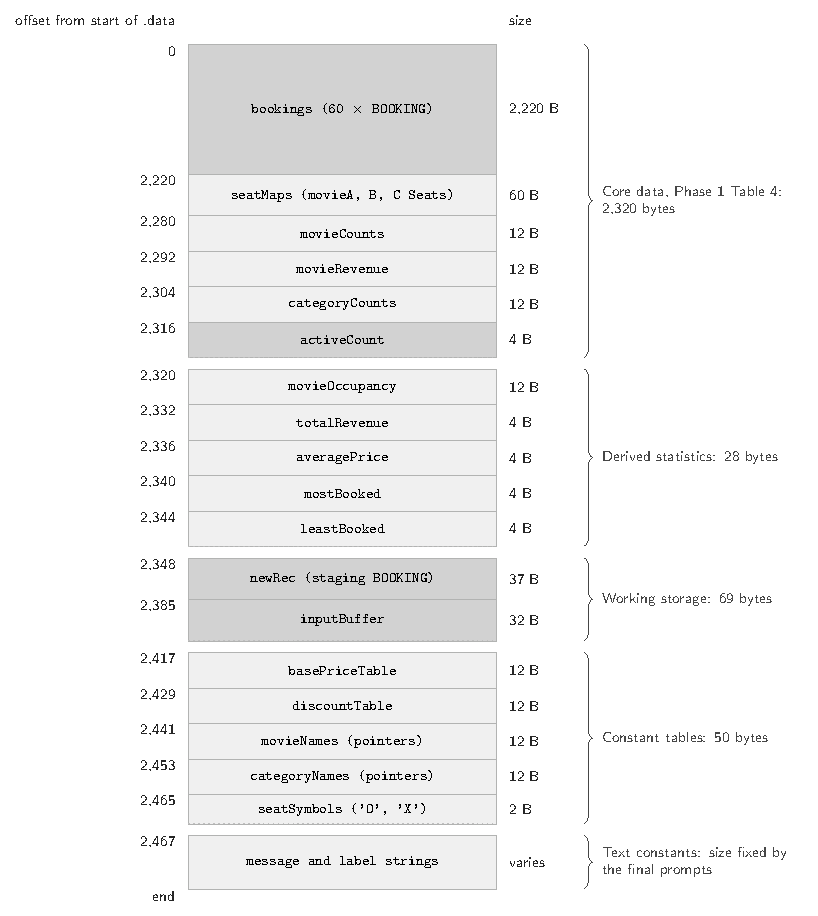
\includegraphics[height=0.75\textheight,width=0.9\textwidth,keepaspectratio]{diagrams/memory-map.pdf}
\caption{Memory map of the data segment: variables in declaration order with offsets and sizes.}
\label{fig:memory}
\end{figure}

\begin{table}[H]
\centering
\tablefont
\caption{Memory totals by group, compared with Phase 1}
\label{tab:memtotals}
\begin{tabular}{|L{0.30\linewidth}|L{0.40\linewidth}|r|}
\hline
\textbf{Group} & \textbf{Contents} & \textbf{Bytes} \\
\hline
Core data (Phase 1 Table 4) & bookings, seat maps, movieCounts, movieRevenue, categoryCounts, activeCount & 2,320 \\
\hline
Derived statistics & movieOccupancy, totalRevenue, averagePrice, mostBooked, leastBooked & 28 \\
\hline
Working storage & newRec (37), inputBuffer (32) & 69 \\
\hline
Constant tables & basePriceTable, discountTable, movieNames, categoryNames, seatSymbols & 50 \\
\hline
\textbf{Fixed total} & & \textbf{2,467} \\
\hline
\end{tabular}
\end{table}

The message strings (menu, prompts, error messages and report labels) follow the tables. Their size depends on the final wording, so it is measured in Phase 3, but it is about one kilobyte. The whole data segment therefore stays near 3.5 KB, well inside the memory of any lab machine. Because the core data and the derived statistics are contiguous (offsets 0 to 2,347), \texttt{Initialize} clears them all with one \texttt{REP STOSB} of 2,348 bytes.

\subsection*{Data segment declaration}

\begin{lstlisting}
MAX_BOOKINGS    = 60
SEATS_PER_MOVIE = 20
NUM_MOVIES      = 3
BUF_SIZE        = 32

.data
; ---- core data (Phase 1 Table 4) ----------------------- offset
bookings        BOOKING MAX_BOOKINGS DUP(<>)            ;     0
seatMaps        LABEL BYTE
movieASeats     BYTE SEATS_PER_MOVIE DUP(0)             ; 2,220
movieBSeats     BYTE SEATS_PER_MOVIE DUP(0)             ; 2,240
movieCSeats     BYTE SEATS_PER_MOVIE DUP(0)             ; 2,260
movieCounts     DWORD NUM_MOVIES DUP(0)                 ; 2,280
movieRevenue    DWORD NUM_MOVIES DUP(0)                 ; 2,292
categoryCounts  DWORD 3 DUP(0)                          ; 2,304
activeCount     DWORD 0                                 ; 2,316
; ---- derived statistics ---------------------------------
movieOccupancy  DWORD NUM_MOVIES DUP(0)                 ; 2,320
totalRevenue    DWORD 0                                 ; 2,332
averagePrice    DWORD 0                                 ; 2,336
mostBooked      DWORD 0                                 ; 2,340
leastBooked     DWORD 0                                 ; 2,344
; ---- working storage ------------------------------------
newRec          BOOKING <>                              ; 2,348
inputBuffer     BYTE BUF_SIZE DUP(0)                    ; 2,385
; ---- constant tables ------------------------------------
basePriceTable  DWORD 8, 7, 6                           ; 2,417
discountTable   DWORD 0, 1, 2                           ; 2,429
movieNames      DWORD OFFSET strMovieA, OFFSET strMovieB, OFFSET strMovieC
categoryNames   DWORD OFFSET strAdult, OFFSET strStudent, OFFSET strChild
seatSymbols     BYTE 'O', 'X'                           ; 2,465
; ---- strings (examples) ---------------------------------
strMovieA       BYTE "Movie A", 0
msgCapacity     BYTE "ERROR: Cinema capacity reached!", 0
msgDuplicateID  BYTE "ERROR: Booking ID already exists!", 0
msgMovieFull    BYTE "ERROR: Movie is full!", 0
msgSeatTaken    BYTE "ERROR: Seat already reserved!", 0
msgNotFound     BYTE "ERROR: Booking ID not found!", 0
\end{lstlisting}

This declaration uses all five data types the brief requires: strings (names and messages), DWORDs (IDs, prices, counters), bytes (movie codes, seats, categories, flags, seat maps), characters (\texttt{seatSymbols}) and arrays (records, seat maps and statistics).

\section{Register Usage Convention}

Table~\ref{tab:registers} fixes the role of each general-purpose register. It follows Appendix D of the brief. The one addition is that EBX also carries a movie code into the seat procedures, since there it is used as a base index into \texttt{seatMaps}, which is the Appendix D role of EBX.

\begin{table}[H]
\centering
\tablefont
\caption{Register usage convention}
\label{tab:registers}
\begin{tabular}{|c|L{0.25\linewidth}|L{0.58\linewidth}|}
\hline
\textbf{Register} & \textbf{Role (Appendix D)} & \textbf{Use in CTRMS} \\
\hline
EAX & Arithmetic results, integer input and output, return values & Result of every procedure that returns a value (menu choice, ID, movie, seat, category, seat count, final price); value printed by \texttt{WriteDec}; dividend and result of \texttt{MUL} and \texttt{DIV} for occupancy and average price; string length from \texttt{ReadString}. \\
\hline
EBX & Record offsets, temporary base and index values & Movie code (1 to 3) passed to \texttt{ValidateSeat}, \texttt{GetSeatAddress} and \texttt{CountReservedSeats}; zero-based index into the DWORD arrays, as in \texttt{movieCounts[ebx*4]}. \\
\hline
ECX & Loop counters & 60 for record scans, 20 for seat-map scans, 4 rows and 5 columns in the seating map (outer count saved with \texttt{PUSH}), 3 for statistics and histogram rows; byte count for \texttt{REP MOVSB} and \texttt{REP STOSB}; buffer size for \texttt{ReadString}. \\
\hline
EDX & String addresses for \texttt{WriteString}; arithmetic support & Address of every prompt and message for \texttt{WriteString}; buffer address for \texttt{ReadString}; prompt address passed to \texttt{ReadNumber}; high half of the dividend, cleared to 0 before every \texttt{DIV}. \\
\hline
ESI & Source and index pointer while scanning records & Address of the current record in \texttt{FindBookingByID} and \texttt{CalculateStatistics}; address of a found record returned to \texttt{CancelBooking} and \texttt{DisplayTicket}; source of the 37-byte copy; pointer into \texttt{inputBuffer} in \texttt{ReadNumber}. \\
\hline
EDI & Destination pointer or seat-map index & Free slot returned by \texttt{FindFreeSlot} (destination of the copy); seat byte address returned by \texttt{GetSeatAddress}; walking pointer in \texttt{CountReservedSeats} and \texttt{DisplaySeatMap}; destination of \texttt{REP STOSB} in \texttt{Initialize}. \\
\hline
\end{tabular}
\end{table}

EBP is not used, because no procedure builds a stack frame (Section~\ref{sec:params}). ESP is changed only by \texttt{CALL}, \texttt{RET}, \texttt{PUSH} and \texttt{POP}. The carry flag in EFLAGS is used as a one-bit result: 0 means success or found, 1 means invalid or not found.

% ── Chapter 3: Procedure Specifications ─────────────────────────────────────

\printchaptertitle{Procedure Specifications}

\section{Procedure Interface Table}

The design uses 24 procedures, well above the minimum of 8 and the recommended 12. Table~\ref{tab:iface-req} covers the 14 procedures named in the brief, and Table~\ref{tab:iface-help} covers \texttt{main} and the 9 helpers that stop the same code being written more than once. Under the convention in Section~\ref{sec:params}, a procedure restores every register it uses, so the \emph{Modified registers} column lists only its outputs. Changes to memory are listed under outputs.

\begin{table}[H]
\centering
\tablefont
\caption{Procedure interface: procedures required by the brief}
\label{tab:iface-req}
\begin{tabular}{|L{0.16\linewidth}|L{0.19\linewidth}|L{0.21\linewidth}|L{0.09\linewidth}|L{0.21\linewidth}|}
\hline
\textbf{Procedure} & \textbf{Inputs} & \textbf{Outputs} & \textbf{Modified} & \textbf{Purpose} \\
\hline
Initialize & None & Memory: offsets 0 to 2,347 cleared & None & Clear records, seat maps and counters at start-up \\
\hline
DisplayMenu & Keyboard & EAX = choice 1 to 6 & EAX & Show the menu and return a valid choice \\
\hline
AddBooking & Keyboard; activeCount, seatMaps & Memory: new record, seat byte, activeCount + 1; screen & None & Collect, validate, price and store a booking \\
\hline
ValidateBookingID & Keyboard & EAX = ID, unique among active records & EAX & Read a six-digit ID and reject duplicates \\
\hline
ValidateMovieCode & Keyboard & EAX = movie code 1 to 3 & EAX & Read and range-check a movie code \\
\hline
ValidateSeat & EBX = movie code; keyboard & EAX = free seat 1 to 20 & EAX & Read a seat, check range and availability \\
\hline
CalculateTicketPrice & ESI = record address (movieCode, category set) & EAX = final price; [ESI].basePrice, [ESI].finalPrice written & EAX & Look up base price and discount, compute final price \\
\hline
FindBookingByID & EAX = booking ID & ESI = record address; CF = 0 found, 1 not found & ESI, CF & Linear search for an active record with this ID \\
\hline
CancelBooking & Keyboard & Memory: activeFlag 0, seat byte 0, activeCount $-$ 1; screen & None & Deactivate a booking and release its seat \\
\hline
DisplayTicket & Keyboard & Screen & None & Print one formatted ticket by booking ID \\
\hline
DisplaySeatMap & Keyboard & Screen & None & Print the 4 $\times$ 5 map, reserved count and occupancy \\
\hline
CalculateStatistics & bookings, activeCount & Memory: all statistics arrays and values & None & Rebuild counts, revenue, occupancy, average, most and least booked \\
\hline
DisplayStatistics & None & Screen & None & Print the statistics report \\
\hline
DisplayHistogram & categoryCounts & Screen & None & Print the category distribution with asterisks \\
\hline
\end{tabular}
\end{table}

\begin{table}[H]
\centering
\tablefont
\caption{Procedure interface: main program and helper procedures}
\label{tab:iface-help}
\begin{tabular}{|L{0.16\linewidth}|L{0.19\linewidth}|L{0.21\linewidth}|L{0.09\linewidth}|L{0.21\linewidth}|}
\hline
\textbf{Procedure} & \textbf{Inputs} & \textbf{Outputs} & \textbf{Modified} & \textbf{Purpose} \\
\hline
main & None & None (ends the process) & All & Program entry: initialise, run the menu loop, exit \\
\hline
ReadNumber & EDX = prompt address; keyboard & EAX = value; CF = 0 valid, 1 invalid & EAX, CF & Read a line and convert 1 to 6 digits to an integer \\
\hline
ReadName & Keyboard & inputBuffer = name; EAX = length 1 to 20 & EAX & Read a customer name of valid length \\
\hline
ReadBookingID & Keyboard & EAX = ID 100000 to 999999 & EAX & Read a booking ID in range (no uniqueness check) \\
\hline
ValidateCategory & Keyboard & EAX = category 1 to 3 & EAX & Read and range-check a ticket category \\
\hline
FindFreeSlot & bookings & EDI = address of first inactive record; CF = 1 if none & EDI, CF & Find a slot for a new booking \\
\hline
GetSeatAddress & EBX = movie code, EAX = seat & EDI = address of the seat byte & EDI & Turn a movie and seat into a seat-map address \\
\hline
CountReservedSeats & EBX = movie code & EAX = reserved seats 0 to 20 & EAX & Count reserved seats of one movie \\
\hline
PrintMovieName & EAX = movie code & Screen & None & Print ``Movie A'', ``Movie B'' or ``Movie C'' \\
\hline
PrintCategoryName & EAX = category & Screen & None & Print ``Adult'', ``Student'' or ``Child'' \\
\hline
\end{tabular}
\end{table}

All screen output goes through Irvine32 routines (\texttt{WriteString}, \texttt{WriteDec}, \texttt{WriteChar}, \texttt{Crlf}, \texttt{Clrscr}, \texttt{WaitMsg}), and all keyboard input through \texttt{ReadString}. These routines preserve every register except their documented result, so calling them never breaks the convention above.

\section{Procedure Call Hierarchy}

Figure~\ref{fig:calls} shows which procedures call which, starting from \texttt{main}. It is split into two columns only to fit the page: both columns are calls made by the same \texttt{main}. A procedure drawn with a dashed border has already been expanded elsewhere in the figure. The deepest chain is four calls: \texttt{main} $\rightarrow$ \texttt{AddBooking} $\rightarrow$ \texttt{ValidateBookingID} $\rightarrow$ \texttt{ReadBookingID} $\rightarrow$ \texttt{ReadNumber}. No procedure calls itself, directly or indirectly.

\begin{figure}[H]
\centering
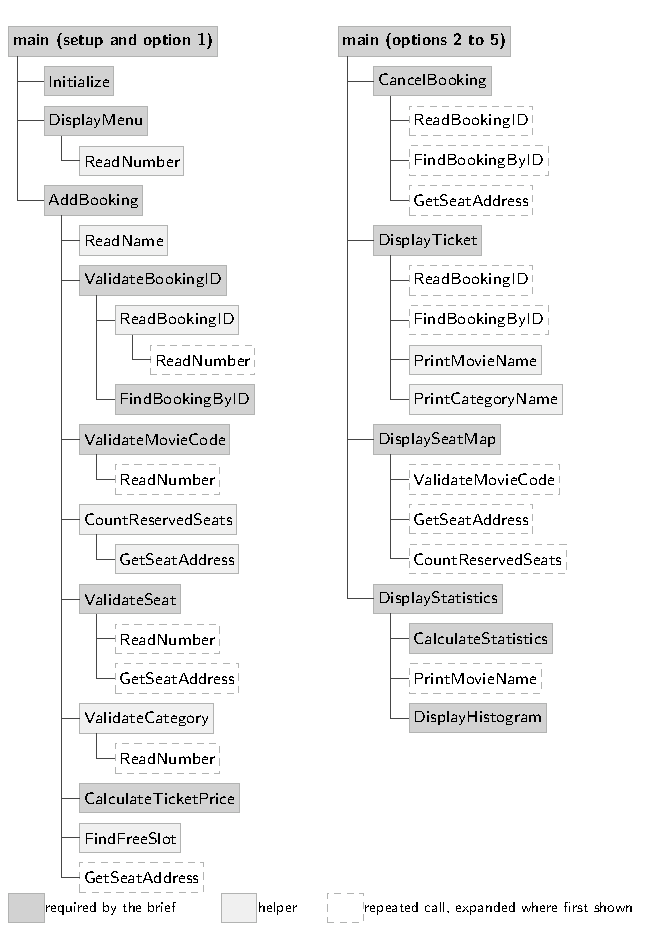
\includegraphics[height=0.72\textheight,width=0.95\textwidth,keepaspectratio]{diagrams/call-hierarchy.pdf}
\caption{Procedure call hierarchy, starting from \texttt{main}.}
\label{fig:calls}
\end{figure}

The hierarchy shows where reuse pays off. \texttt{ReadNumber} is called by five procedures, \texttt{GetSeatAddress} by five, and \texttt{FindBookingByID} and \texttt{ReadBookingID} by three each. Each piece of validation and searching logic therefore exists exactly once in the program.

\section{Parameter Passing Convention}
\label{sec:params}

CTRMS passes parameters in \textbf{registers}. Shared data (the records, seat maps and counters) stays in \textbf{memory} as global variables. The \textbf{stack} is not used for parameters. The rules are:

\begin{enumerate}
\item \textbf{Inputs in registers.} A procedure receives at most two inputs, each in the register given in Tables~\ref{tab:iface-req} and~\ref{tab:iface-help}: EAX for a value, EBX for a movie code, EDX for a string address, ESI for a record address.
\item \textbf{One result in a register.} A value is returned in EAX. An address is returned in ESI (a record found by a search) or EDI (a destination: a free slot or a seat byte).
\item \textbf{Status in the carry flag.} A procedure that can fail sets CF with \texttt{STC} or clears it with \texttt{CLC} just before \texttt{RET}. The caller tests it with \texttt{JC} or \texttt{JNC} straight after the call.
\item \textbf{The callee preserves registers.} Each procedure pushes the registers it uses on entry and pops them in reverse order before \texttt{RET}, except its output registers. A caller can therefore keep a value, such as the movie code in EBX during \texttt{AddBooking}, across any call.
\item \textbf{Shared arrays are global memory.} Procedures read and write \texttt{bookings}, \texttt{seatMaps} and the counters by name. A record is passed \emph{by reference}, as its address in ESI, never by copying its 37 bytes.
\item \textbf{No stack parameters and no stack frames.} The stack holds only return addresses and saved registers, so every procedure ends with a plain \texttt{RET} and EBP is never needed.
\end{enumerate}

\begin{table}[H]
\centering
\tablefont
\caption{Parameter passing methods and where each is used}
\label{tab:passing}
\begin{tabular}{|L{0.17\linewidth}|L{0.11\linewidth}|L{0.31\linewidth}|L{0.31\linewidth}|}
\hline
\textbf{Method} & \textbf{Used?} & \textbf{Where} & \textbf{Example} \\
\hline
Registers (values) & Yes & Every procedure input and result & \texttt{GetSeatAddress}: EBX = movie, EAX = seat, returns EDI \\
\hline
Registers (addresses) & Yes & Record passed by reference, prompt strings & \texttt{CalculateTicketPrice}: ESI = record; \texttt{ReadNumber}: EDX = prompt \\
\hline
Flags & Yes & Found or valid status & \texttt{FindBookingByID}: CF = 1 when not found \\
\hline
Memory (global variables) & Yes & Arrays and counters shared by many procedures & \texttt{activeCount}, \texttt{bookings}, \texttt{seatMaps} \\
\hline
Stack & No & Only return addresses and saved registers & \texttt{PUSH ECX} around the inner loop of \texttt{DisplaySeatMap} \\
\hline
\end{tabular}
\end{table}

\subsection*{Why registers}

\begin{itemize}
\item \textbf{The interfaces are small.} No procedure needs more than two inputs, so the six general-purpose registers are always enough and nothing has to spill onto the stack.
\item \textbf{It matches Irvine32.} The library already takes its arguments in registers (EDX for \texttt{WriteString}, EAX for \texttt{WriteDec}, EDX and ECX for \texttt{ReadString}), so CTRMS procedures and library calls follow one style.
\item \textbf{It is the fastest and simplest.} Registers need no memory access and no stack frame to set up or remove, so a call is just the \texttt{CALL} and the \texttt{RET}.
\item \textbf{The carry flag suits yes-or-no results.} A search or a validation is followed immediately by one conditional jump, without comparing a return code.
\item \textbf{Global arrays avoid copying.} Passing a 2,220-byte array on the stack is impossible in practice, and passing its address to every procedure would add nothing, because there is only one booking array.
\end{itemize}

Stack parameters (\texttt{PROTO} and \texttt{INVOKE}, with \texttt{[EBP+8]} addressing) were considered and rejected. They pay off for libraries called from many programs, or for recursion, and CTRMS needs neither.

\subsection*{Example}

The caller and the callee of \texttt{GetSeatAddress}, as they will appear in Phase 3:

\begin{lstlisting}
; caller (inside ValidateSeat): EBX = movie code, EAX = seat number
    call GetSeatAddress              ; EDI = address of the seat byte
    cmp  BYTE PTR [edi], 1
    je   seatTaken

; callee
GetSeatAddress PROC                  ; in: EBX, EAX   out: EDI
    push eax                         ; preserve the caller's EAX
    mov  edi, ebx
    dec  edi                         ; movie 1..3 -> 0..2
    imul edi, edi, SEATS_PER_MOVIE   ; x 20
    dec  eax                         ; seat 1..20 -> 0..19
    add  edi, eax
    add  edi, OFFSET seatMaps
    pop  eax
    ret
GetSeatAddress ENDP
\end{lstlisting}

\section{Coverage of the Technical Requirements}

Table~\ref{tab:coverage} checks the design against the technical requirements in Section 2.4 of the brief, so that the code review in Phase 3 has a list to work from.

\begin{table}[H]
\centering
\tablefont
\caption{Technical requirements and where the design meets them}
\label{tab:coverage}
\begin{tabular}{|L{0.25\linewidth}|L{0.67\linewidth}|}
\hline
\textbf{Requirement} & \textbf{Where in the design} \\
\hline
At least 2 loop structures & \texttt{LOOP} with ECX: \texttt{FindBookingByID}, \texttt{FindFreeSlot}, \texttt{CountReservedSeats}, \texttt{CalculateStatistics}, \texttt{DisplaySeatMap}. \texttt{JMP}-based while loops: \texttt{main}, \texttt{DisplayMenu}, \texttt{ReadNumber}, every \texttt{Validate} procedure, the histogram stars. \texttt{REP} string loops: \texttt{Initialize}, the record copy in \texttt{AddBooking}. \\
\hline
IF & Capacity and full-movie checks in \texttt{AddBooking}; leading zero for seats below 10 in \texttt{DisplaySeatMap}. \\
\hline
IF-ELSE & Found or not found in \texttt{CancelBooking} and \texttt{DisplayTicket}; average price with or without bookings in \texttt{CalculateStatistics}; the dispatch chain in \texttt{main}. \\
\hline
Nested conditionals & Range check then availability check in \texttt{ValidateSeat}; active flag then ID match in \texttt{FindBookingByID}. \\
\hline
At least 8 procedures & 24 procedures (Tables~\ref{tab:iface-req} and~\ref{tab:iface-help}). \\
\hline
Strings, DWORDs, bytes, characters, arrays & Section 2.3: names and messages; IDs, prices and counters; codes, seats and flags; \texttt{seatSymbols}; records, seat maps and statistics. \\
\hline
Fixed-size records & \texttt{BOOKING}, 37 bytes, reached by index $\times$ 37 + field offset (Section 2.1). \\
\hline
Validation before writing & Every field is validated into \texttt{newRec}; the record is copied into \texttt{bookings} only after the last check (Section 1.2). \\
\hline
No floating point & Prices use \texttt{SUB}; occupancy and average use \texttt{MUL} and \texttt{DIV} on unsigned integers. \\
\hline
\end{tabular}
\end{table}

\end{document}
